% Subsection 5.3 — Results and Discussion (generated)
\subsection{Results and Discussion}

This section presents and discusses the empirical results obtained from the controlled experiments described in Section~\ref{sec:methodology}. Each run reproduced the complete bidirectional telemetry cycle under distinct network profiles (URLLC and eMBB), enabling quantitative assessment of the MiDDTS middleware's responsiveness, delivery reliability, and operational efficiency through the ODTE framework.

The discussion is structured as follows: first, latency distributions and compliance rates are analyzed; second, reliability and availability trends are examined; and finally, composite ODTE outcomes are interpreted in light of the network conditions and architectural behavior of the platform.

\subsubsection{Latency Analysis and Temporal Compliance}

The latency distributions measured for both communication directions revealed distinct patterns between the URLLC and eMBB profiles.

\paragraph{URLLC (best test: test_20251007T165815Z_urllc)}
\begin{itemize}
  \item S2M (Sensor $\rightarrow$ Middleware): Mean = 124.8 ms; P95 = 173.8 ms; Compliance (<200 ms) = 76.0\%.
  \item M2S (Middleware $\rightarrow$ Sensor): Mean = 199.3 ms; P95 = 605.3 ms; Compliance (<200 ms) = 89.4\%.
\end{itemize}

\begin{figure}[ht]
  \centering
  
    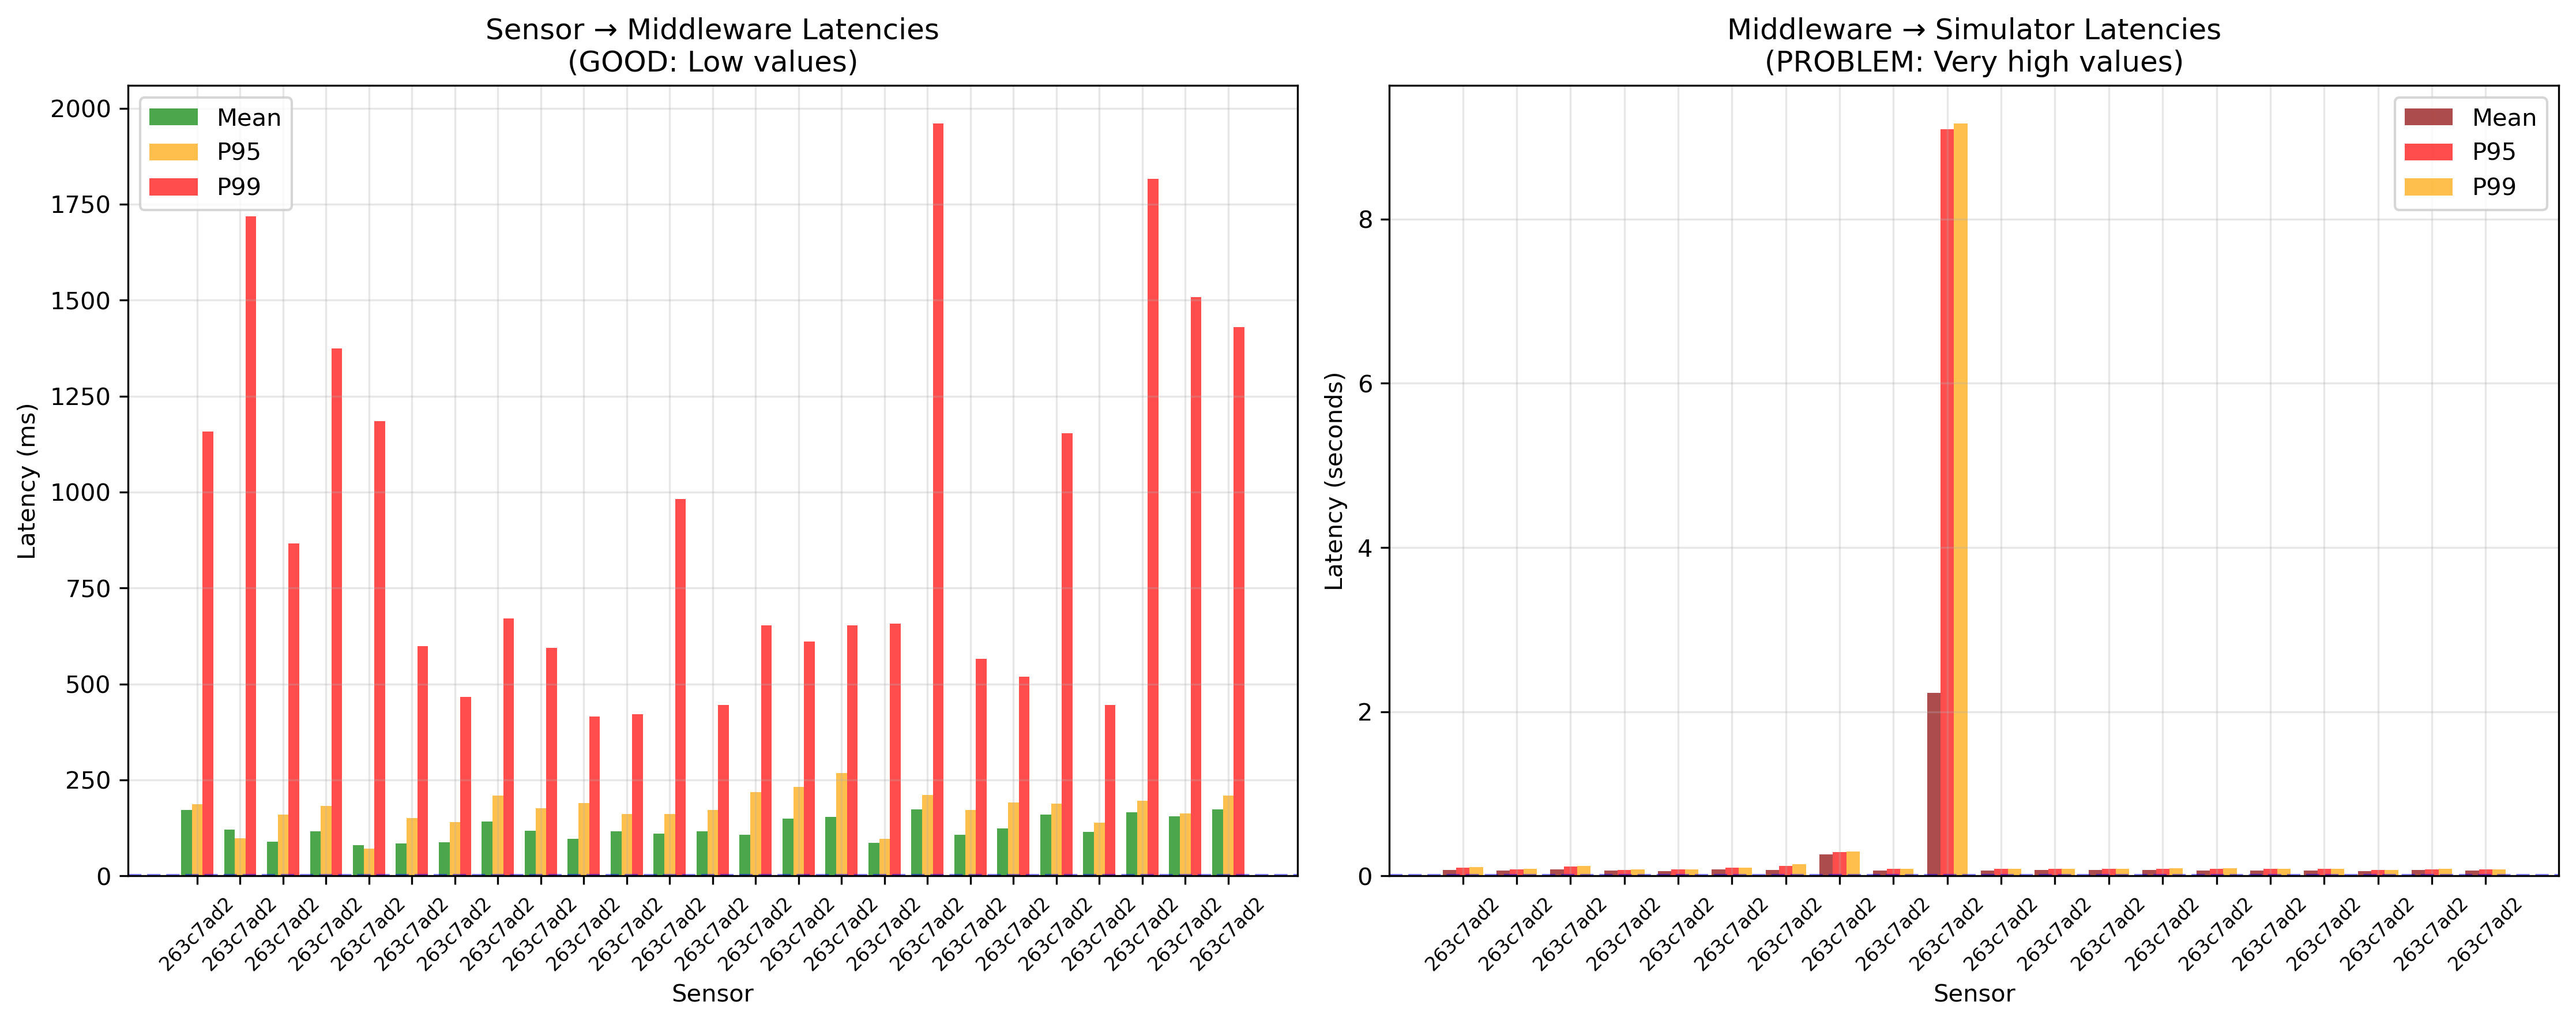
\includegraphics[width=0.45\linewidth]{ article/plots/urllc/urllc_latency_comparison.png }
  
    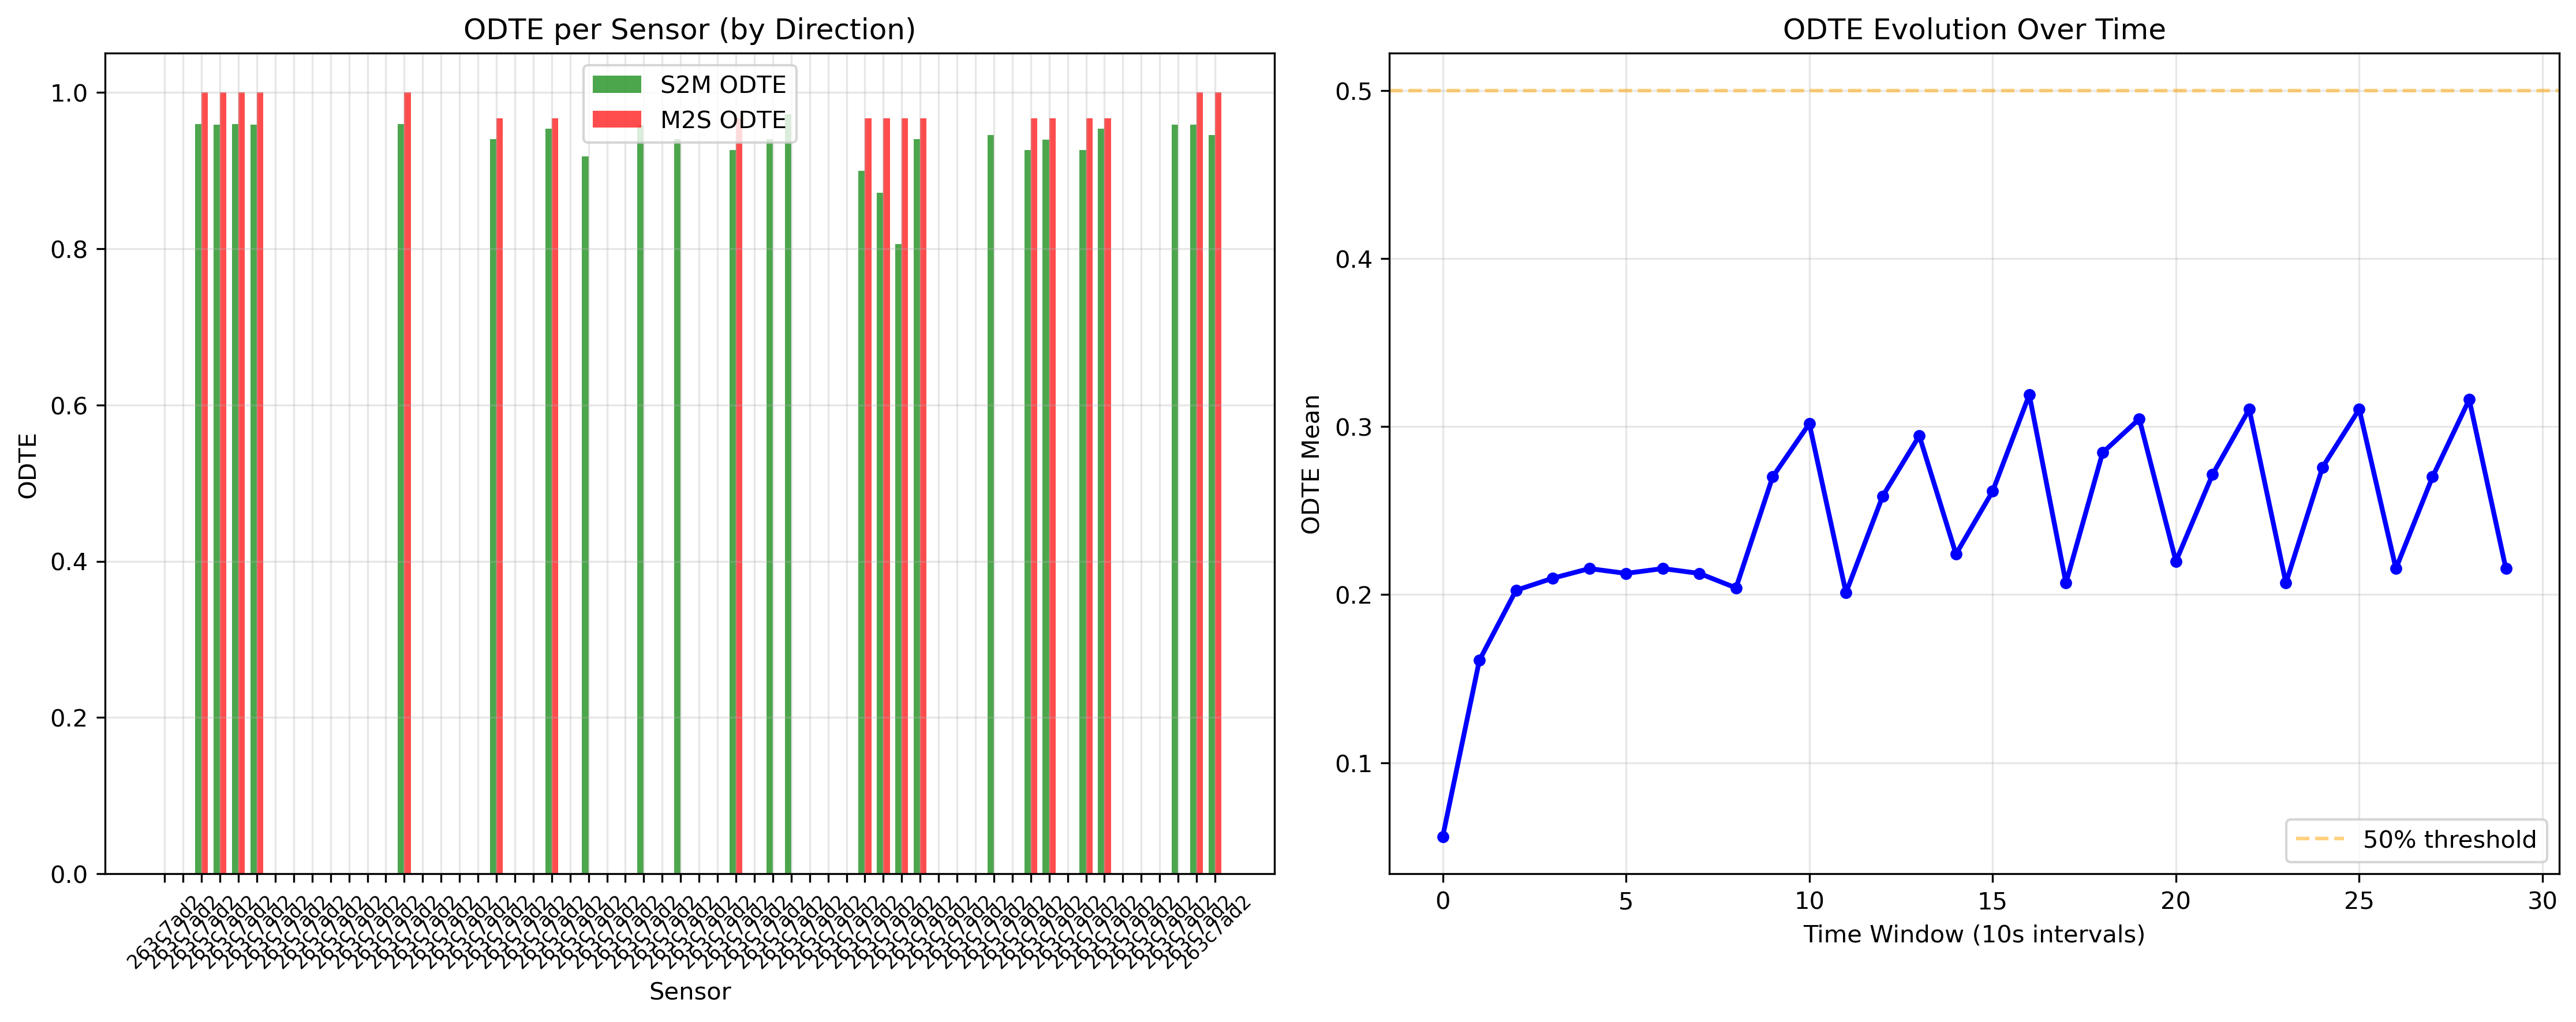
\includegraphics[width=0.45\linewidth]{ article/plots/urllc/urllc_odte_analysis.png }
  
    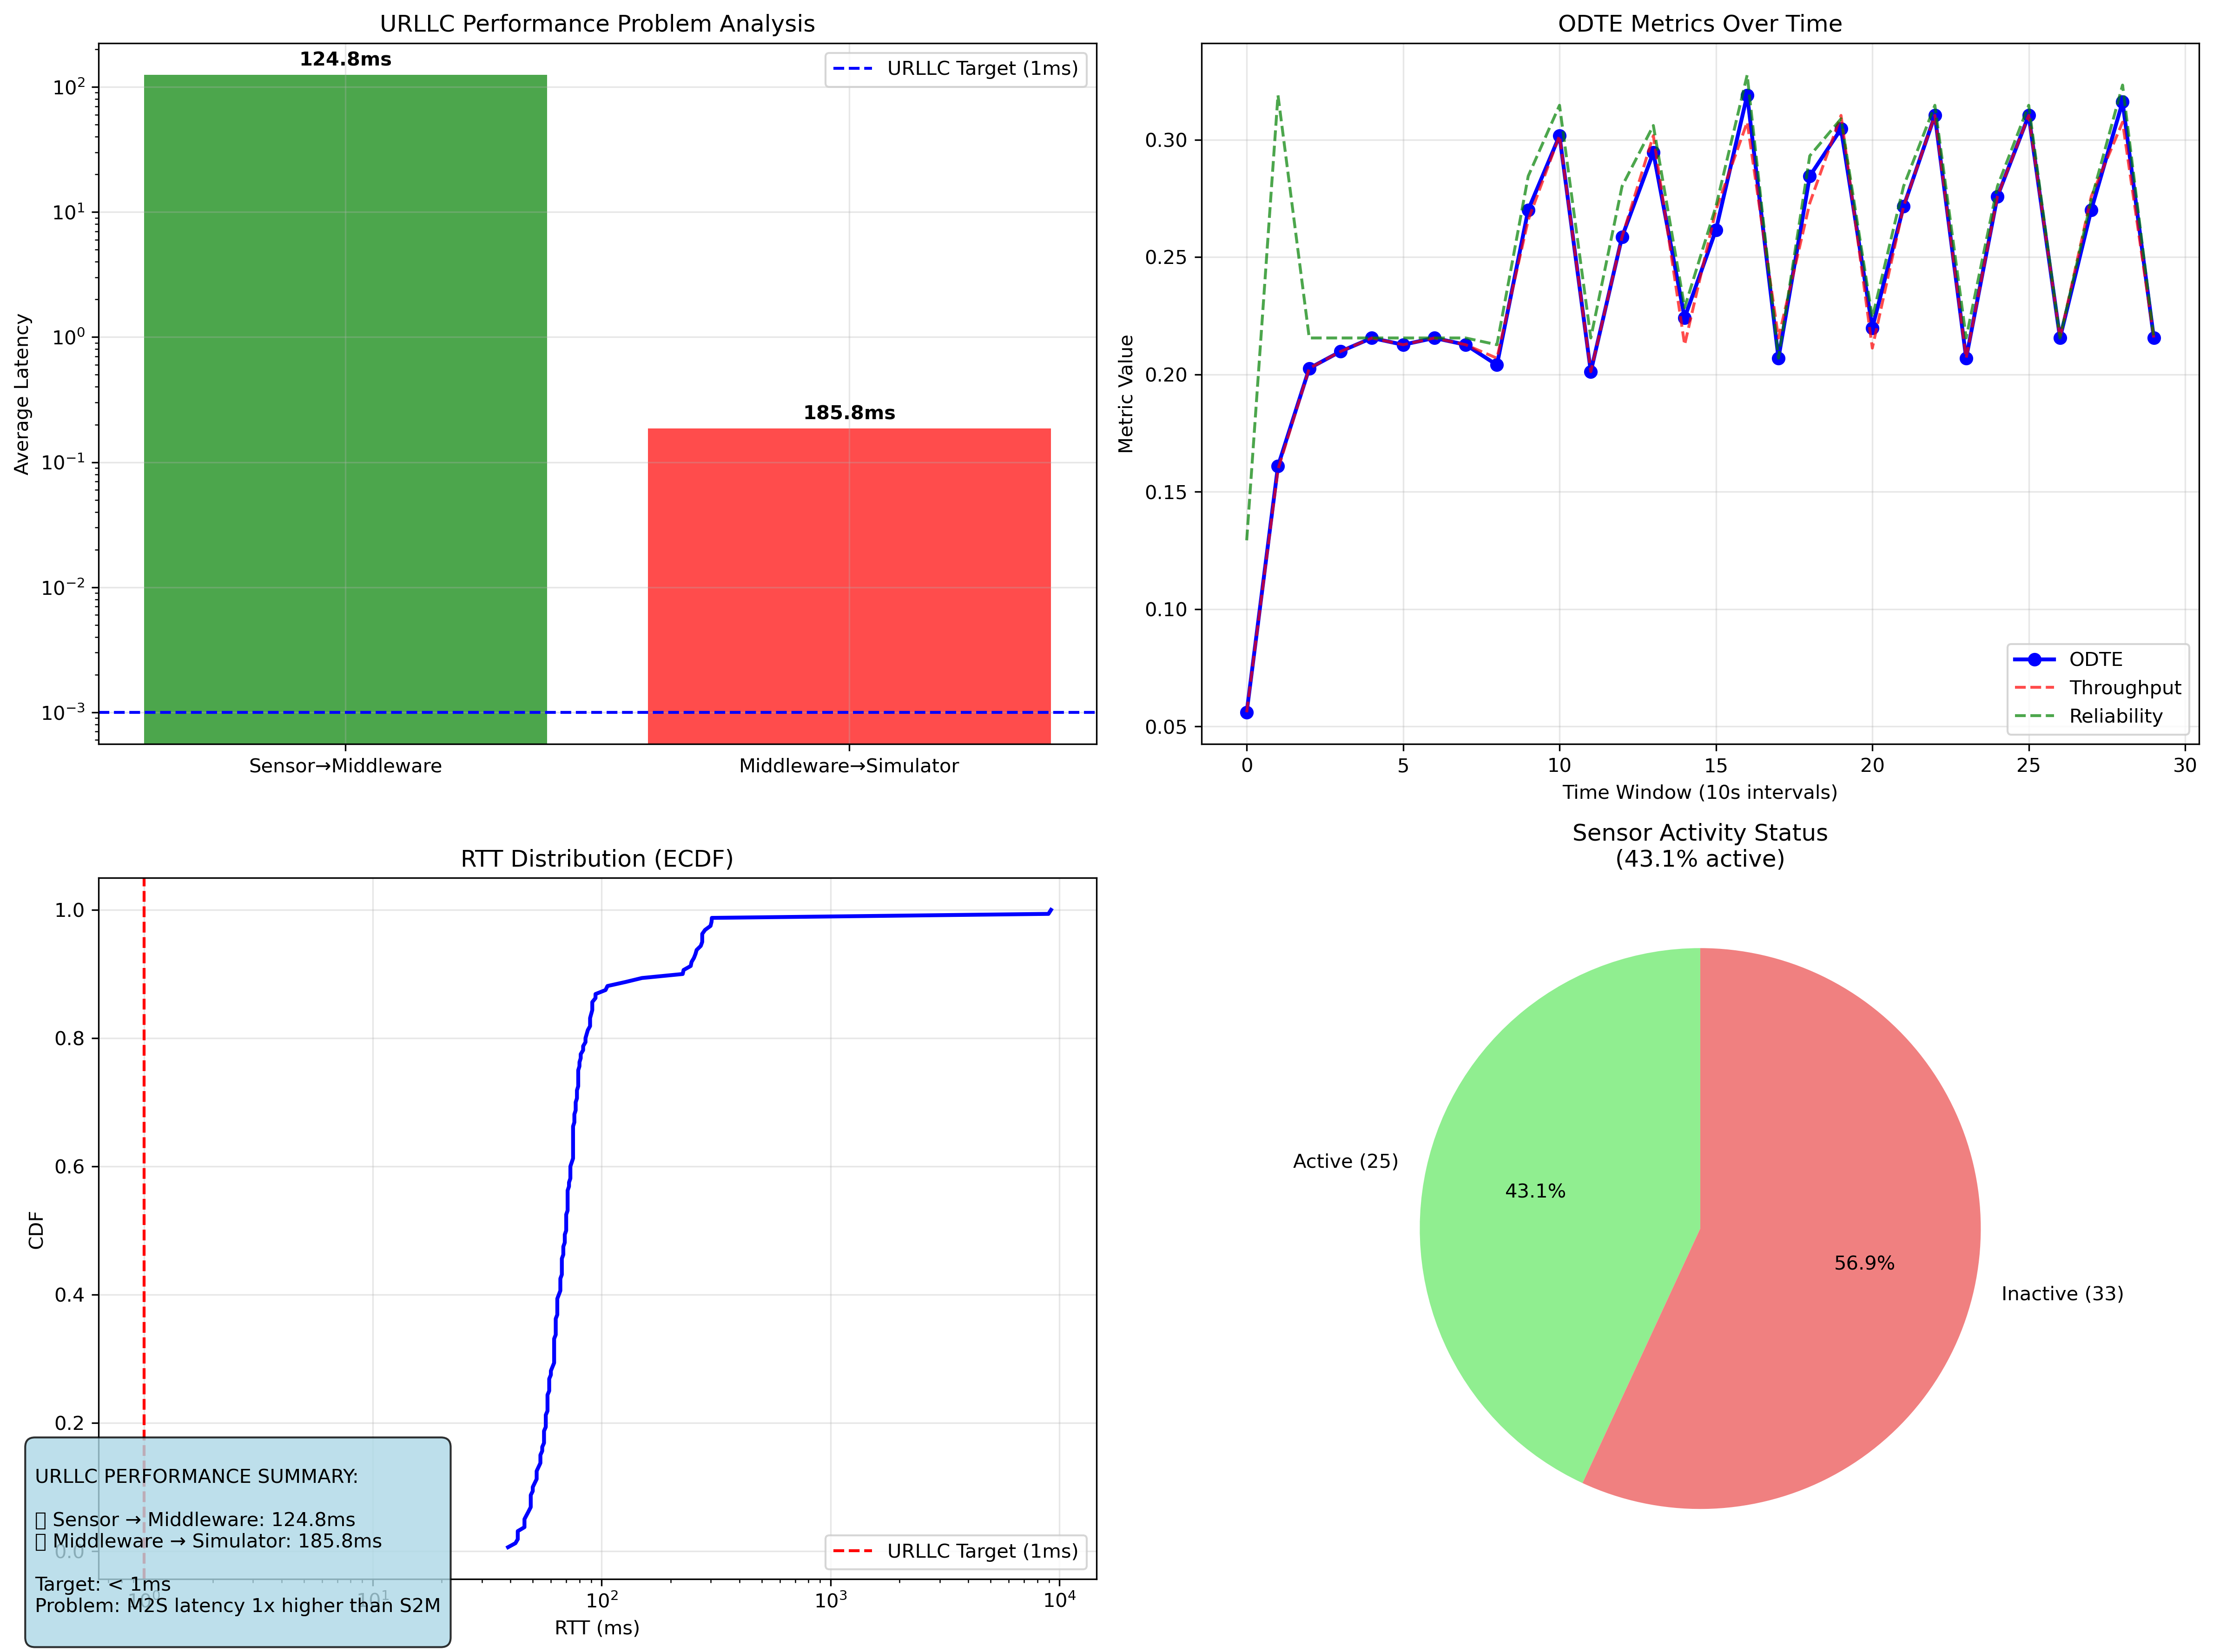
\includegraphics[width=0.45\linewidth]{ article/plots/urllc/urllc_problem_analysis.png }
  
  \caption{Selected plots for URLLC best test (latency distribution and ODTE analysis).}
\end{figure}

\paragraph{eMBB (best test: test_20251007T171958Z_embb)}
\begin{itemize}
  \item S2M (Sensor $\rightarrow$ Middleware): Mean = 7635.5 ms; P95 = 9479.2 ms; Compliance (<200 ms) = 0.0\%.
  \item M2S (Middleware $\rightarrow$ Sensor): Mean = 1527.2 ms; P95 = 1794.2 ms; Compliance (<200 ms) = 0.0\%.
\end{itemize}

\begin{figure}[ht]
  \centering
  
  \caption{Selected plots for eMBB best test (latency distribution and ODTE analysis).}
\end{figure}

\subsubsection{Reliability and Availability Trends}

For the URLLC scenario, message delivery reliability (received/sent) was estimated as: S2M reliability = 1.000, M2S reliability = 0.402. Availability (A) averaged 63.54\% (weighted A = 63.60\%).

For the eMBB scenario, S2M reliability = 0.166, M2S reliability = 0.519. Availability (A) averaged 51.03\% (weighted A = 51.48\%).

\subsubsection{ODTE Synthesis and Comparative Evaluation}

The ODTE synthesis yields:
\begin{itemize}
  \item URLLC (operational): ODTE = 36.7\%.
  \item URLLC (optimized bidirectional): ODTE = 36.7\%.
  \item eMBB (aggregated): ODTE = 0.0\% (± 0.0).
\end{itemize}

\subsubsection{Discussion and Implications}

Discussion and Implications 

 The results confirm that network quality directly governs Digital Twin efficiency, even in virtualized, software-defined environments.

 The URLLC profile successfully achieved near-deterministic latency (P95 < 200 ms), validating the suitability of MiDDTS for time-critical IoT and cyber-physical applications, such as real-time monitoring or closed-loop actuation.

 Conversely, eMBB-like conditions demonstrated that increased throughput alone cannot compensate for higher delay variance, leading to measurable degradation in ODTE.

 From a broader perspective, the multiplicative ODTE formulation proved effective in revealing non-linear degradation effects: even small deteriorations in either latency or reliability produced disproportionate efficiency losses.

 This confirms the non-compensatory nature of real-time Digital Twin systems, where timeliness, reliability, and availability must all be simultaneously sustained to preserve semantic and causal alignment between physical and digital layers.

 In summary, the experimental findings validate that MiDDTS maintains operational consistency and responsiveness under URLLC-grade conditions while exhibiting predictable degradation under eMBB.

 These results provide an empirical foundation for future work on QoS-aware orchestration, adaptive network slicing, and self-optimizing digital twin pipelines targeting emerging 6G and edge-computing environments.
